% MUMmer Whole Genome Comparisons
%
% Basic MUMmer genome comparison example

\subsection{MUMmer Whole Genome Comparisons}
\begin{frame}
  \frametitle{MUMmer}
  \begin{itemize}
    \item \texttt{MUMmer} is a suite of alignment programs and scripts
    \begin{itemize}
      \item \texttt{mummer}, \texttt{promer}, \texttt{nucmer}, etc.
    \end{itemize}
    \item Very different to BLAST (suffix tree alignment) - very fast
    \item Extremely flexible
    \item Used for genome comparisons, assemblies, scaffolding, repeat detection, etc.
    \item Forms the basis for other aligners/assemblers
  \end{itemize}
\end{frame}

% [fragile] frames must end with \end{frame} directly following a newline, or they break!
\begin{frame}[fragile]
  \frametitle{Run a MUMmer Comparison}
  Create a new sub-directory for MUMmer output.
\begin{lstlisting}[language=bash]
$ cd ~/introToBioinformatics/data/workshop
$ mkdir nucmer_out
\end{lstlisting}
    Run \texttt{nucmer} to create \texttt{chrA\_NC\_004547.delta} \\
\begin{lstlisting}[language=bash]
$ nucmer --prefix=nucmer_out/chrA_NC_004547 chrA.fasta NC_004547.fna
\end{lstlisting}
    Then filter this file to generate a coordinate table for visualisation
\begin{lstlisting}[language=bash]
$ delta-filter -q nucmer_out/chrA_NC_004547.delta > nucmer_out/chrA_NC_004547.filter
$ show-coords -rcl nucmer_out/chrA_NC_004547.filter > nucmer_out/chrA_NC_004547_filtered.coords
\end{lstlisting}
\end{frame}

% [fragile] frames must end with \end{frame} directly following a newline, or they break!
\begin{frame}[fragile]
  \frametitle{Run a MUMmer Comparison}
  MUMmer output is very different from BLAST output
\begin{lstlisting}[language=bash]
$ head nucmer_out/chrA_NC_004547_filtered.coords
...
\end{lstlisting}
\end{frame}

% [fragile] frames must end with \end{frame} directly following a newline, or they break!
\begin{frame}[fragile]
  \frametitle{Run a MUMmer Comparison}
  Use a one-line shell command to convert to \texttt{ACT}-friendly format:
\begin{lstlisting}[language=bash]
$ tail -n +6 nucmer_out/chrA_NC_004547_filtered.coords | awk '{print $7" "$10" "$1" "$2" "$12" "$4" "$5" "$13}' > chrA_mummer_NC_004547.crunch
$ head chrA_mummer_NC_004547.crunch 
2526 82.49 15 2540 4727782 4985117 4982588 5064019
2944 82.29 2676 5619 4727782 4982544 4979600 5064019
85 95.29 11092 11176 4727782 758690 758774 5064019
1356 81.69 17446 18801 4727782 77639 78994 5064019
\end{lstlisting}
\end{frame}

\subsubsection{Viewing Alignments}
\begin{frame}
  \frametitle{Select Files}    
  Select your chromosome, and the megaBLAST/MUMmer output
  \begin{center}
    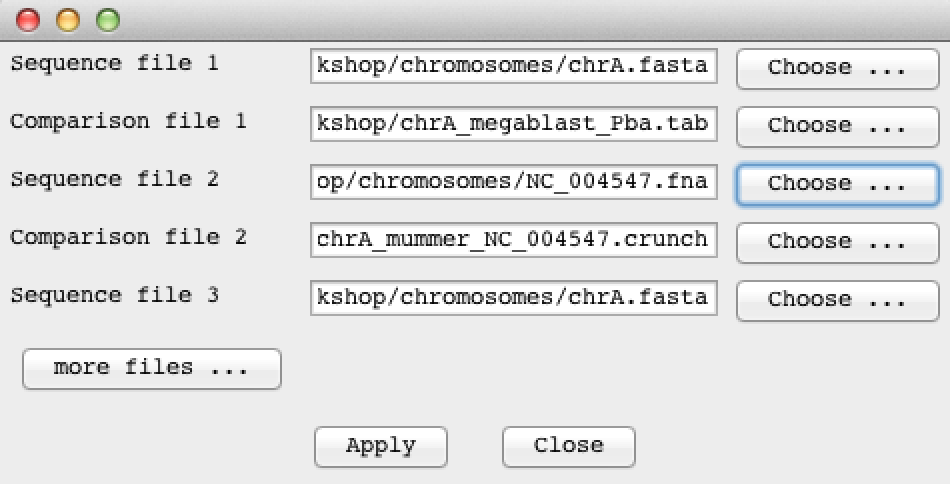
\includegraphics[width=0.9\textwidth]{images/act_wgs8}     
  \end{center}
\end{frame}

\begin{frame}
  \frametitle{View Basic Alignment}    
  \begin{center}
    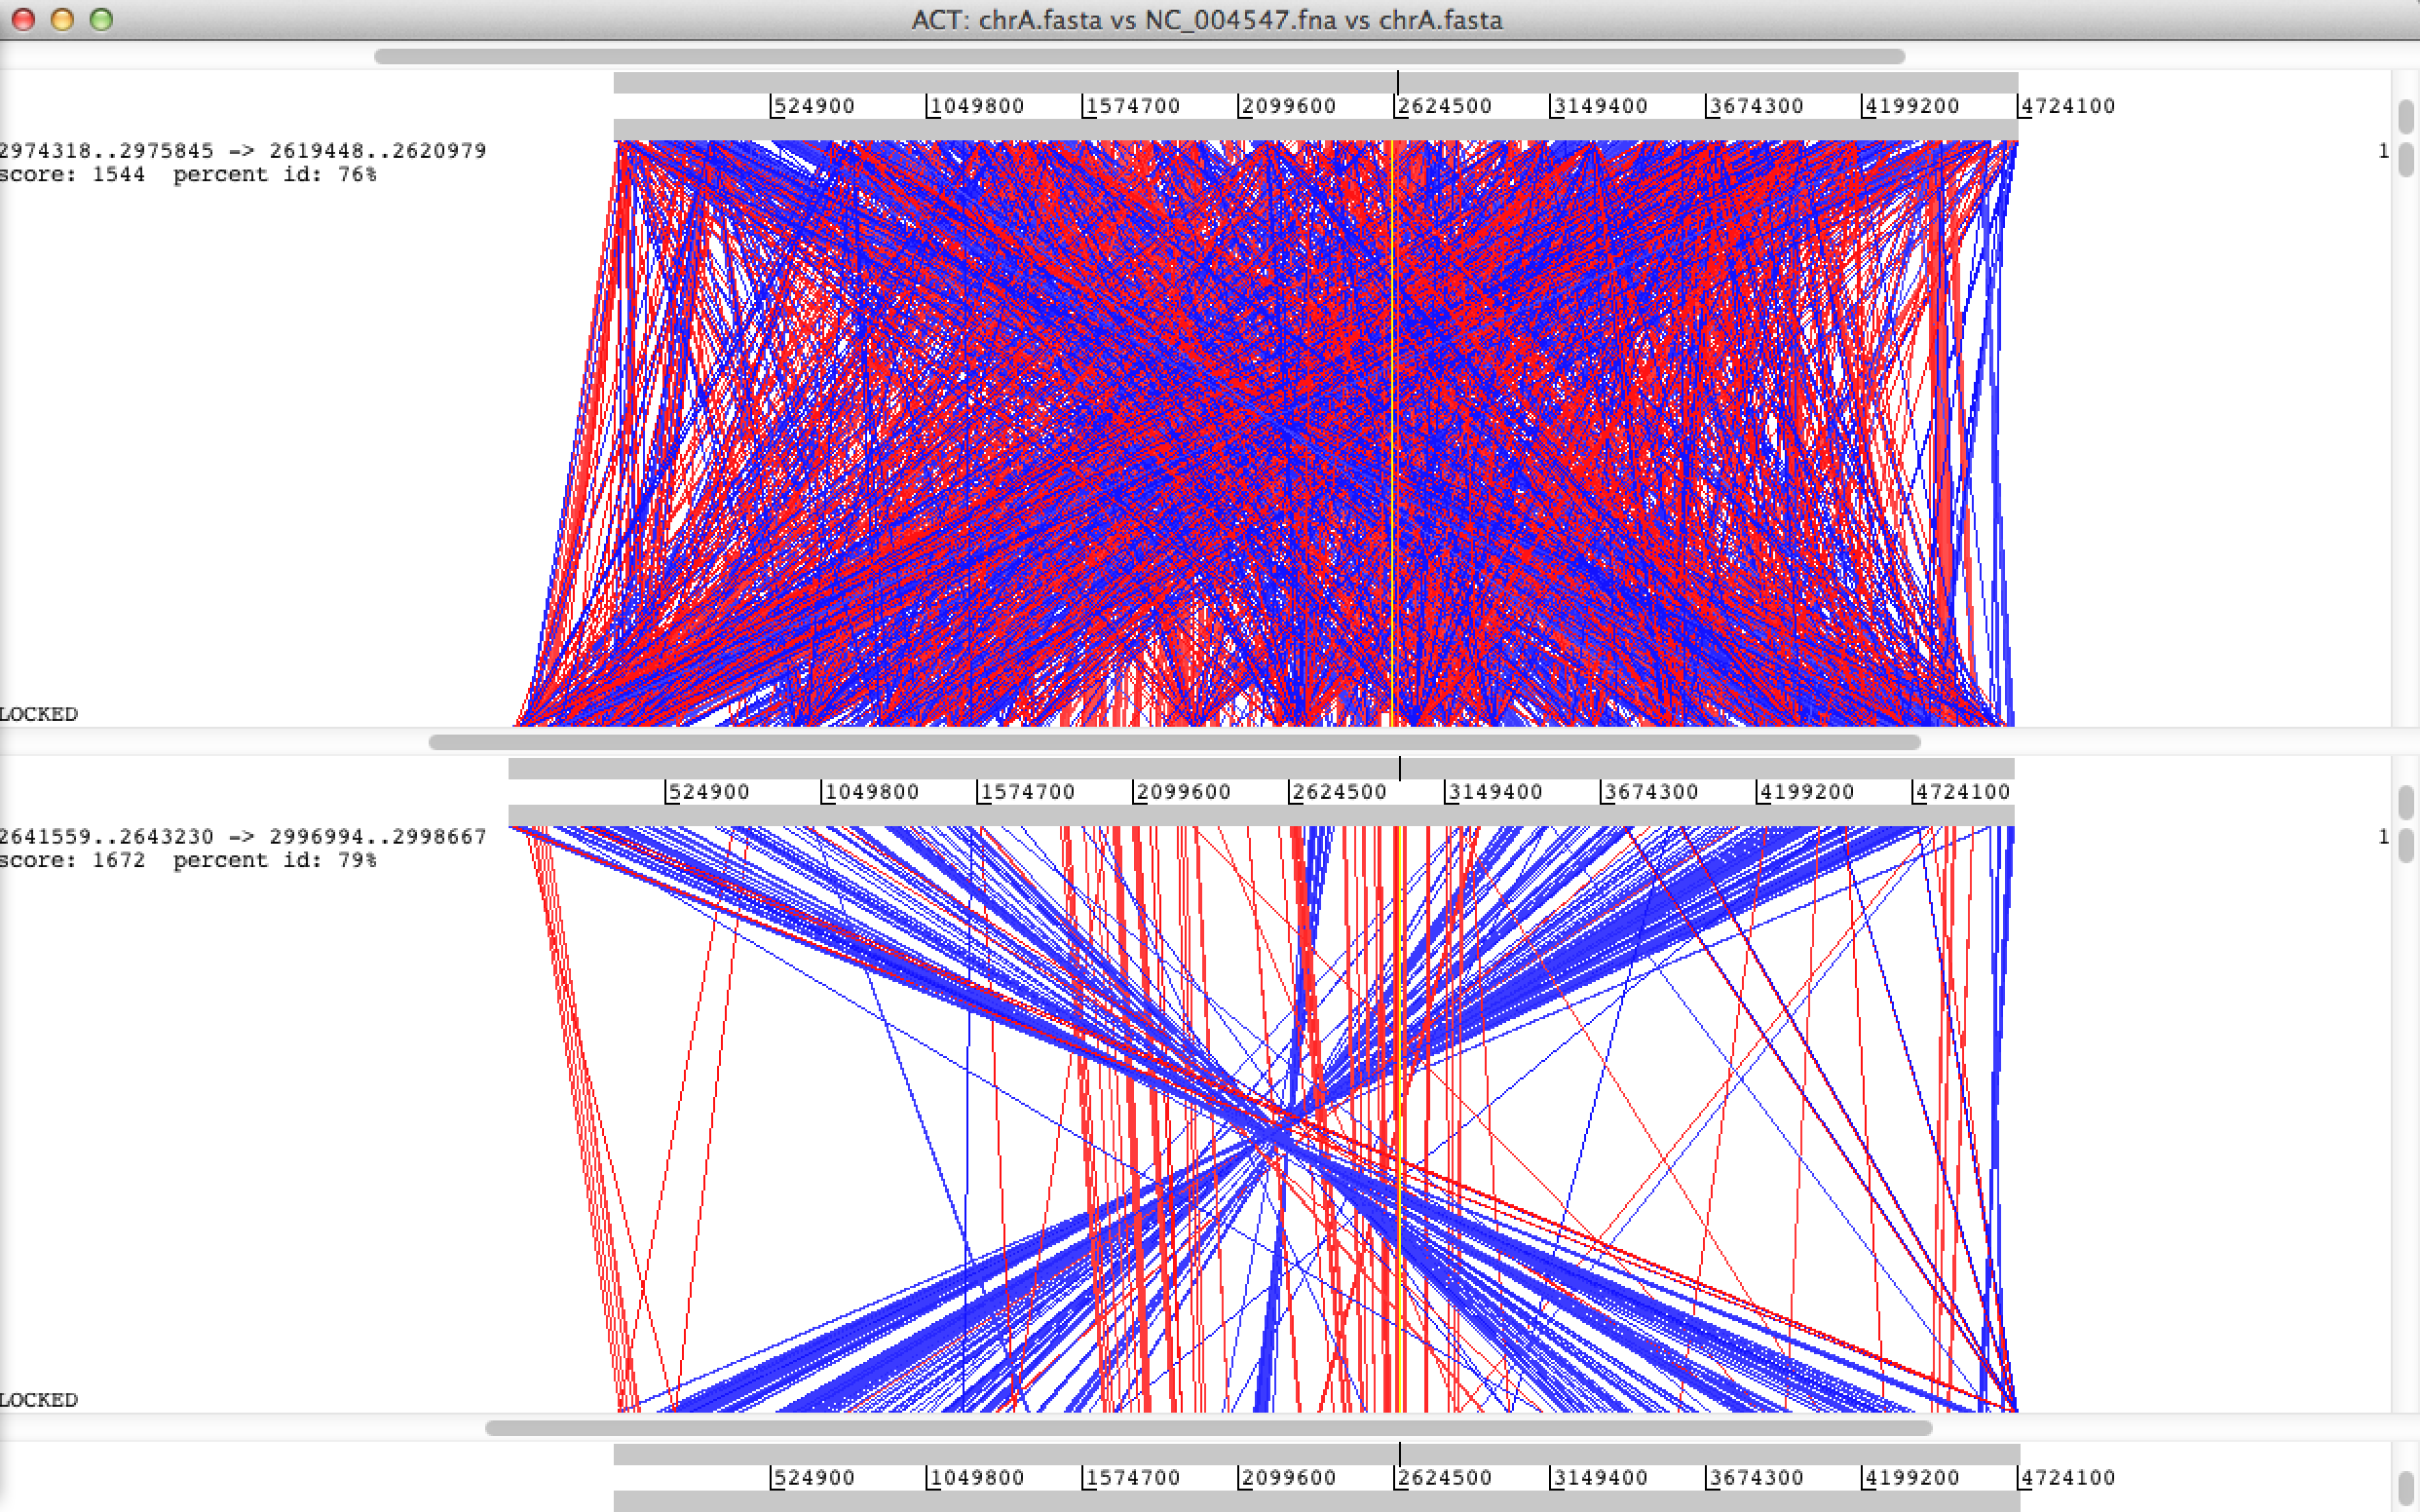
\includegraphics[width=0.8\textwidth]{images/act_wgs9}     
  \end{center}
\end{frame}

\begin{frame}
  \frametitle{Filter Weak BLAST Matches}    
  \begin{center}
    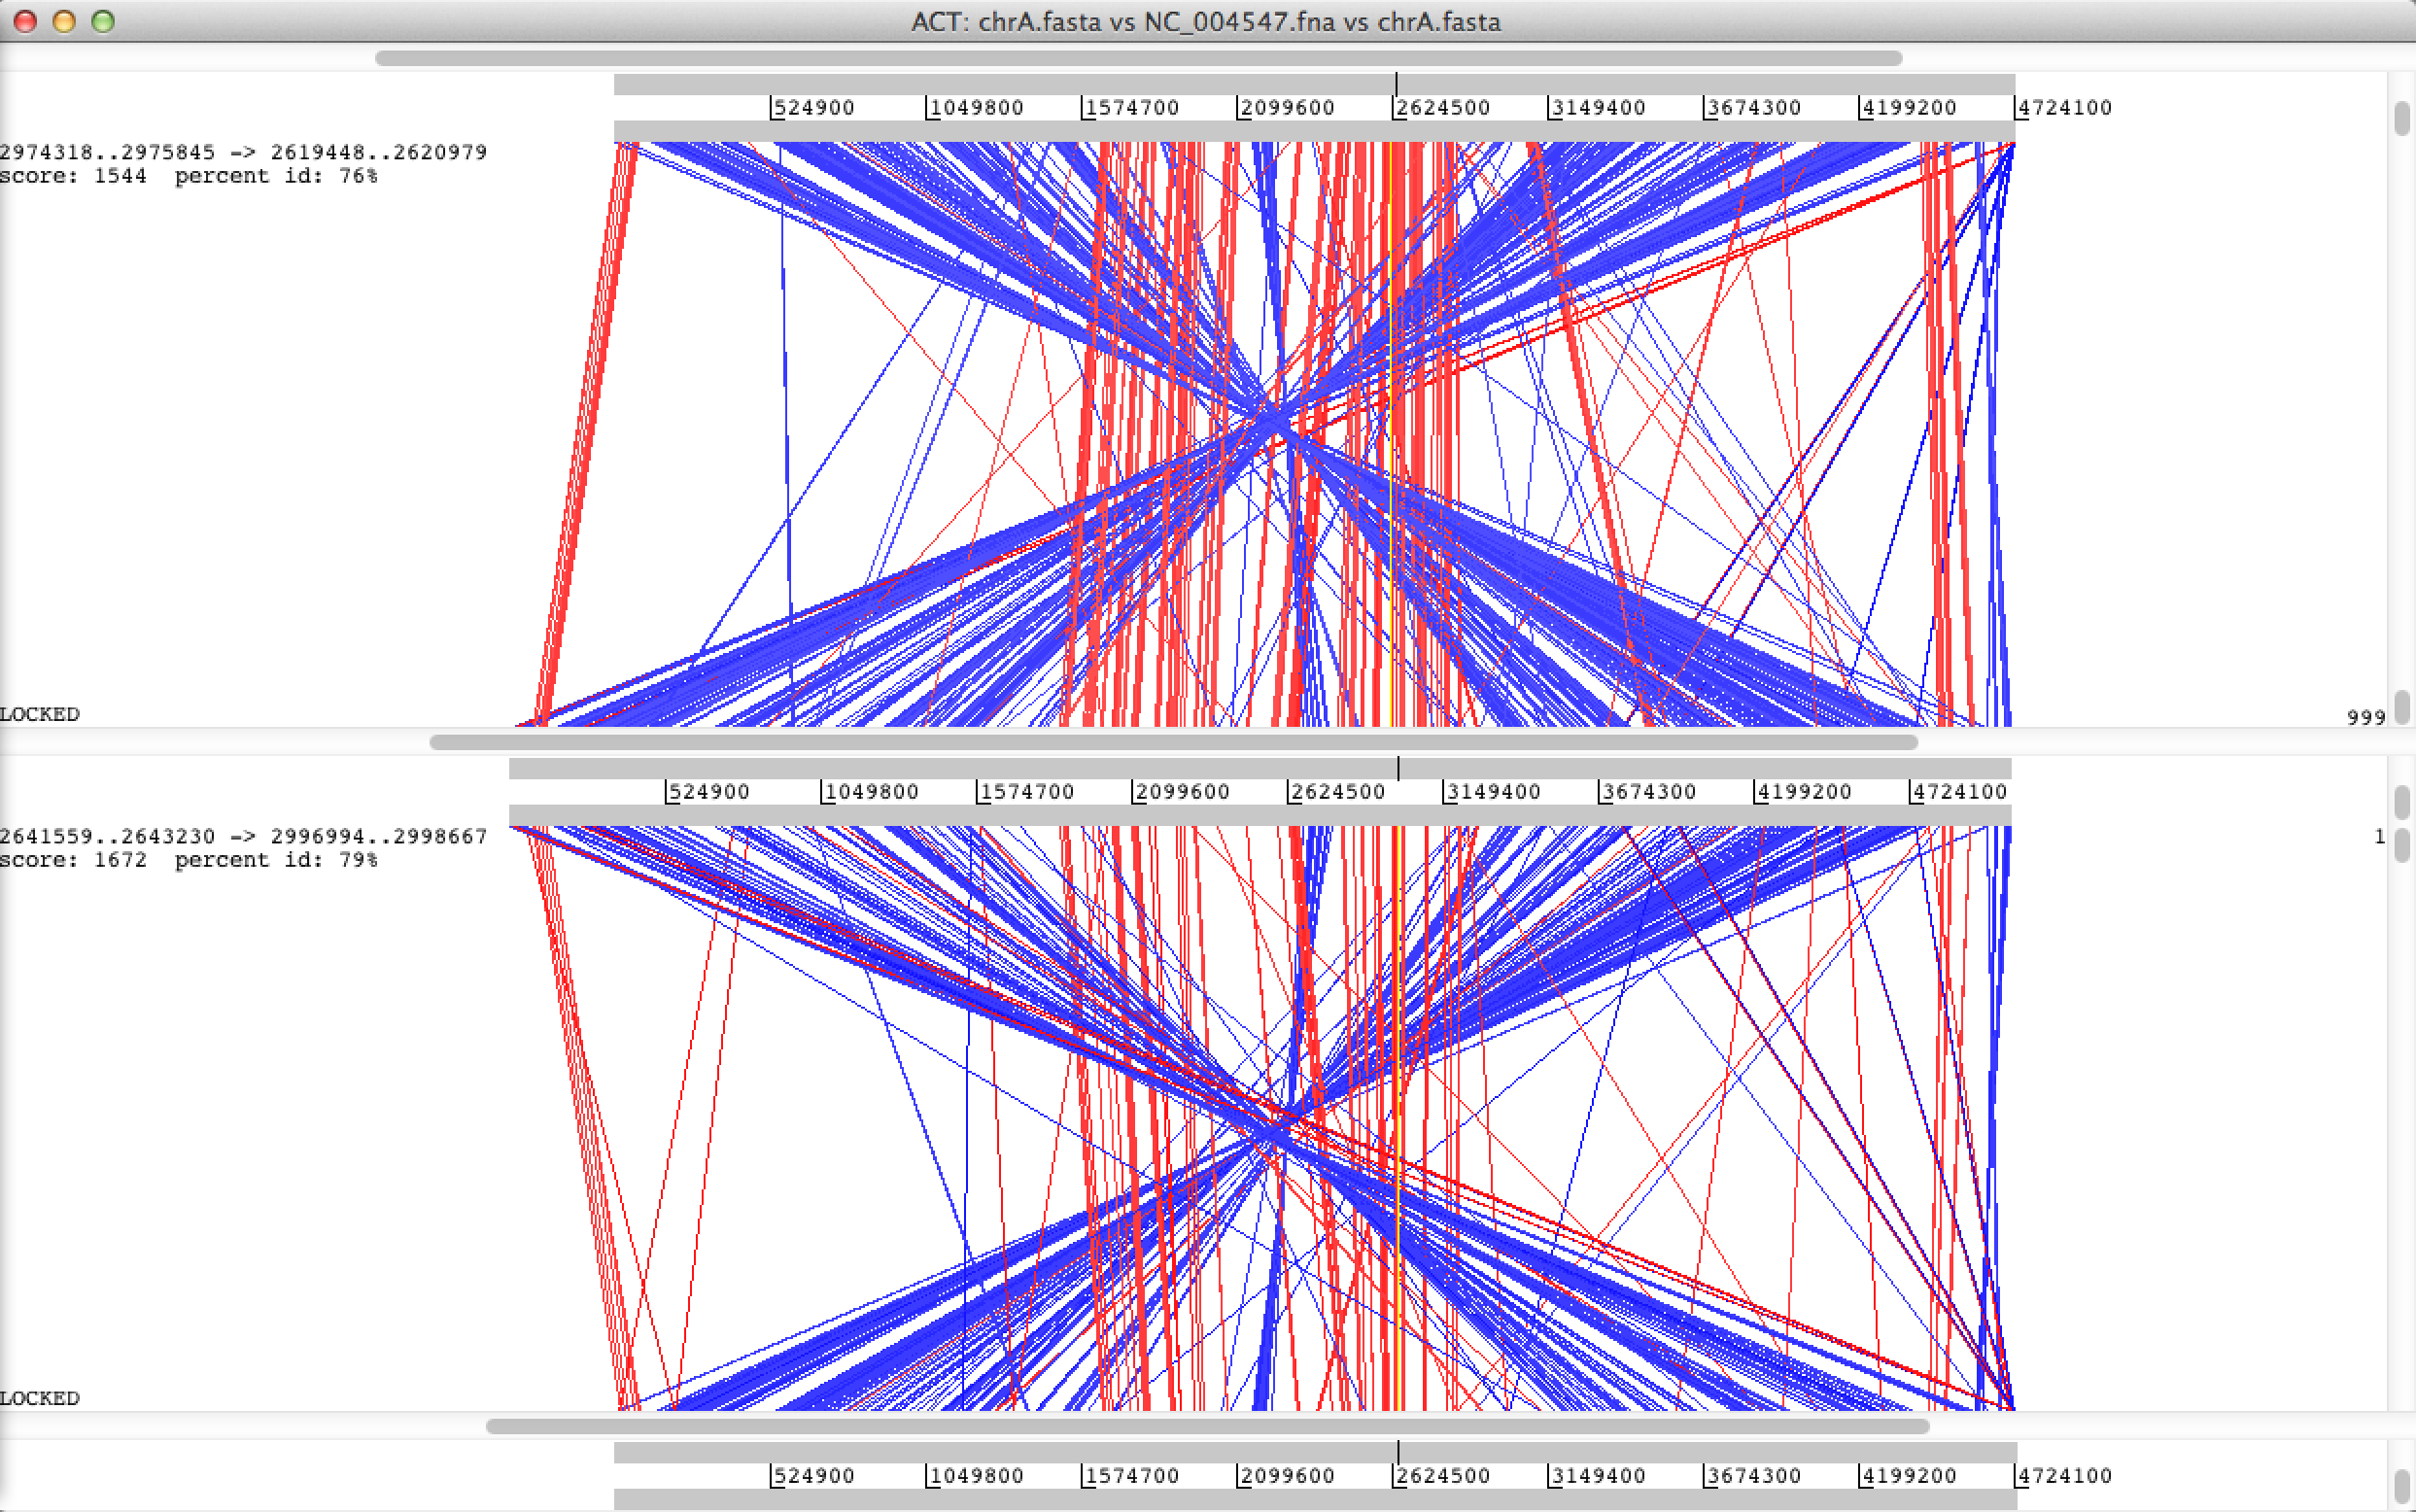
\includegraphics[width=0.8\textwidth]{images/act_wgs10}     
  \end{center}
\end{frame}
